\label{sec:hitbox}
Hitbox $H_o \approx K_o$ ist eine Approximation für ein Modell in einer Simulation. Sie abstrahieren das konkrete Modell dabei für einige oder gar alle physikalischen Berechnungskontexte. Prinzipiell sind exakte Modelle $K_o$, bzw.~$G_o$ ebenfalls Hitboxen.\\
Der Term Hitbox suggeriert die Verwendung einer Box/eines Quaders zur Approximation. Das ist wahrscheinlich historisch bedingt. Der Term Hitbox ist allerdings auch für andere Formen etabliert.\\
Die Diskrepanz zwischen Hitbox und Model $\mathcal{D}(H_o) = | H_o \cup K_o \backslash (H_o \cap K_o) |$ wirkt sich negativ auf den physikalischen Realismus aus, da so False Positives/Negatives  in z.B.~Kollisionsroutinen entstehen.\\
Eine vereinfachte Darstellung eines Modells durch eine Hitbox mag jedoch Berechnungsvorteile bieten.\\
Mehrere Hitboxen können zu einem Objekt angegeben sein $H_{o, [i]}$. Dafür können mehrere Gründe angegeben werden:
\begin{enumerate}
\item Um komplexere Hitboxen durch Komposition darzustellen $H_{o, [ges]} = \bigcup_{\forall i}H_{o, [i]}$
\item Um durch verschachtelte Hitboxen so ein Objekt räumlich sukzessiv zu approximieren.
Typischerweise soll dann eine Ordnung nach der Diskrepanz $H_{o, [i]} < H_{o, [j]} \Leftrightarrow \mathcal{D}(H_{o, [i]}) < \mathcal{D}(H_{o, [j]})$ gelten. Die Hitbox mit der geringsten Diskrepanz, die Hitbox $H_{o, [min]}=min\{H_{o, [i]}\}$, wenn modellgenau $H_{o, [min]} = K_o$, wird dann als finale Hitbox bezeichnet.
\end{enumerate}

\begin{figure*}
	\begin{subfigure}[t]{0.45\textwidth}
		\centering
		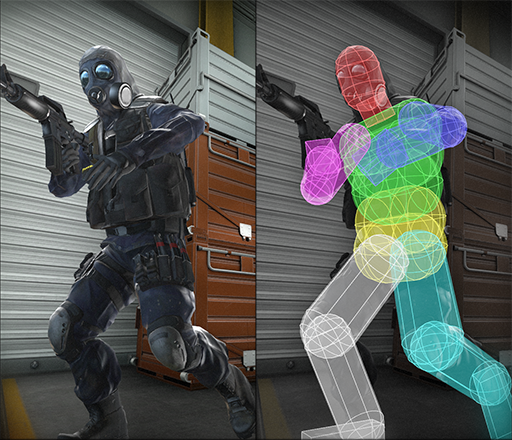
\includegraphics[width=1\textwidth]{./res/csgo_hitbox.png}
		\caption{Hitbox des Spieler-Modells aus dem Videospiel Counter Strike: Global Offensive; sichtbares Modell(links), mit eingeblendeten Hitboxen (rechts)}
%%TODO source for pic
		\label{fig:chitbox}
	\end{subfigure}
~
	\begin{subfigure}[t]{0.2\textwidth}
		\centering
		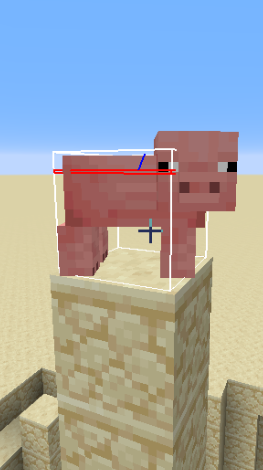
\includegraphics[width=1\textwidth]{./res/pig_hitbox.png}
		\caption{Hitbox eines NPC-Modells (Schwein) aus dem Videospiel Minecraft; Hitbox in weiß}
		\label{fig:mphitbox}
	\end{subfigure}
~
	\begin{subfigure}[t]{0.2\textwidth}
		\centering
		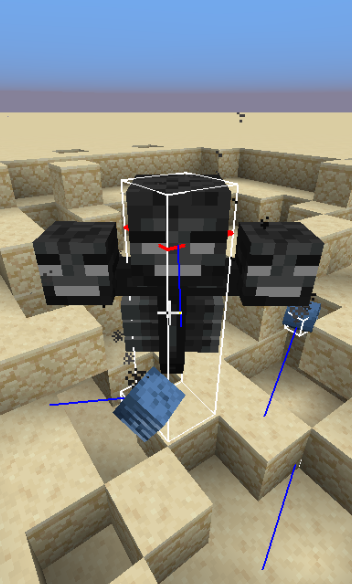
\includegraphics[width=1\textwidth]{./res/wither_hitbox.png}
		\caption{Hitbox eines NPC-Modells (Wither) aus dem Videospiel Minecraft; Hitbox in weiß}
		\label{fig:mwhitbox}
	\end{subfigure}

	\caption{Güten von Hitboxen}
	\label{fig:hitbox}
\end{figure*}

Die Abbildungen~\ref{fig:hitbox} zeigen Hitboxen in 2 verschiedenen Spielen die die kreativen Freiheitsgrade bei der Wahl von Hitboxen und ihrer Diskrepanzen verdeutlichen sollen.\\
\ref{fig:chitbox} zeigt das Spielermodell aus dem Spiel Counter-Strike: Global Offensive (CSGO). Die angezeigten Hitboxen sind hier Ellipsoide.
Die Partition in einzelne Hitboxen für ein Modell ist ebenfalls zu erkennen.
Einzelne Details des Spielermodells, wie Riemen und Taschen an der Ausrüsung, sind im Spiel nicht essentiell und werden daher auch physikalisch nicht abgebildet.\\
Die Partition der Hitboxen in CSGO ergibt sich direkt aus einer Anforderung der Anwendung, Schusstreffer auf verschiedene Teile des Spielermodells unterschiedlich zu bewerten. Beispielsweise verursacht der Treffer am Kopf am meisten Schaden. CSGO modelliert die unterschiedlichen treffbaren Teile des Modells also über mehrere Hitboxen.\\
CSGO ist ein Shooter. Schnelle Reaktion und genaues Zielen sind ein Hauptbestandteil des Produkts. Zudem ist CSGO ein hoch kompetitiver E-Sport, der professionell gespielt wird. Es geht dabei um Preisgelder im siebenstelligen Bereich \cite{csgoprice}. Akkurate und, aus der perspektive des Spielers deterministische Hitboxen sind daher essenziell für das Produkt.\\
Abbildungen~\ref{fig:mphitbox} und~\ref{fig:mwhitbox} zeigen Hitboxen aus dem Spiel Minecraft bei zwei Nicht-Spieler-Charakteren. Die hohe Diskrepanz ist merklich. Mehr noch: Die Minecraft-Hitboxen sind koordinatenachsenparallel, d.h. Kanten verlaufen immer entlang der Koordinatenachsen der Raumrepräsentation und drehen sich nicht bei der Drehung des Modells.\\
Minecraft ist ein Sandbox Aufbauspiel. Ziel des Spiels ist der Bau von beliebigen Gebäuden, Tunneln, die Kreation von Maschinen, das Erkunden von Gebieten und was dem Spieler sonst noch einfällt.\\
In Minecraft steckt auch eine erhebliche Summe Geld. Am 15. September 2014 kaufte Microsoft die Entwicklerfirma und die rechte am Spiel für ca. 2,5 Milliarden Dollar \cite{buyminecraft}.\\
Minecraft ist nicht mit Fokus für schnelle Spieler-gegen-Spieler Szenarien kreiert. Die gesamte Spielwelt ist aus sichtbaren achsenparallel aufgestellten Würfeln aufgebaut, welche durch achsenparallele Hitboxen perfekt abgebildet werden können. Minecraft macht es sich weiter offenbar einfach und verwendet diese an Modellen wieder. Tatsächlich werden künstlich kleinere Hitboxen manchmal sogar eingesetzt um einen Treffer künstlich zu erschweren (vgl. Abbildung \ref{fig:mwhitbox}).\\
Vielleicht mag eine indirekt proportionale Korrelation zwischen der Diskrepanz bei Hitboxen und Erfolg bestehen, jedoch kann die Kritikalität von Diskrepanz nicht in allen Fällen bestätigt werden.
